
\subsection{Definition}

A \textbf{branch-and-bound} algorithm consists of a systematic enumeration of candidate solutions by means of state space search: the set of candidate solutions is thought of as forming a rooted tree with the full set at the root. The algorithm explores branches of this tree, which represent subsets of the solution set. Before enumerating the candidate solutions of a branch, the branch is checked against upper and lower estimated bounds on the optimal solution, and is discarded if it cannot produce a better solution than the best one found so far by the algorithm.

\subsection{Solving the knapsack problem with B\&B}

Given the following knapsack problem :

\begin{figure}[!ht]
    \centering
    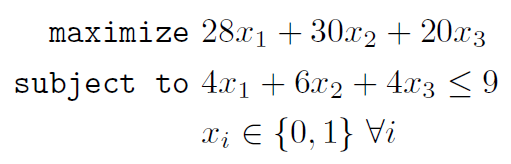
\includegraphics[width=0.4\linewidth]{KnapsackBBProblem.png}
    \label{fig:Knapsack_example}
\end{figure}
\FloatBarrier

We can choose to relax either of the constraint during the branch and bound procedure 
as to obtain a solution. The goal being to reduce the search space as much as possible
by calculating an upper bound as precise as possible.
Let us thus compare both options in the following sections.

\subsubsection{Capacity relaxation}

The first constraint that we can relax is the capacity constraint. The B\&B
calculation becomes fairly simple to implement as we only cut at tree branch when 
we have surpassed the capacity. The search space is thus reduced as such :

\begin{figure}[!ht]
    \centering
    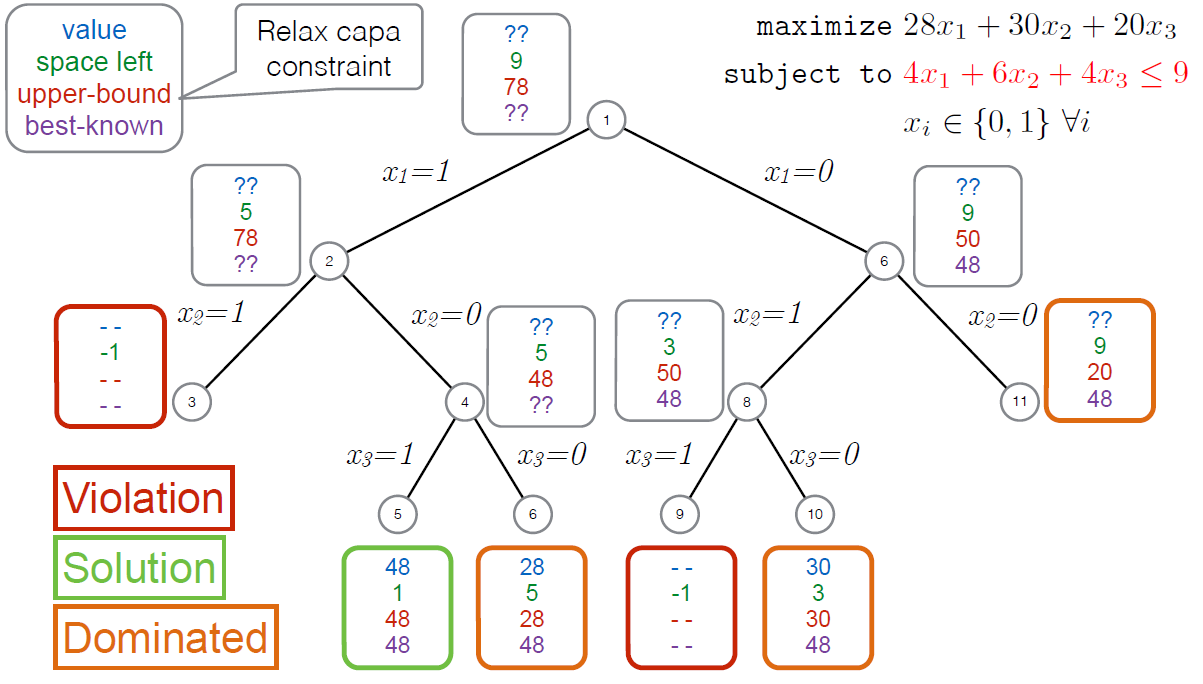
\includegraphics[width=\linewidth]{KnapsackBBCapaRelaxation.png}
    \label{fig:Knapsack_example}
\end{figure}
\FloatBarrier

Which, as you can see, is far from optimal as our upper bound are not close enough to their
real value.

\subsubsection{Linear relaxation}

This second relaxation is slightly harder to implement but yields better result, as 
the upper bound approximation is far better. Given a set sorted by ratio $v_i/w_i$,
the upper bound calculation procedure become as search for the first critical item j.
\newline

The first critical item j being the first item which cannot be fully added in our selection
due to capacity constraint. 

\begin{figure}[!ht]
    \centering
    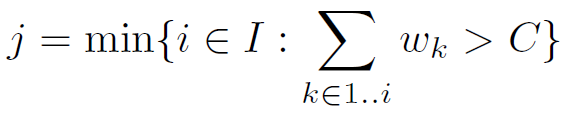
\includegraphics[width=0.4\linewidth]{KnapsackBBCriticalItem.png}
    \label{fig:Knapsack_example}
\end{figure}
\FloatBarrier

The upper bound can then be calculated as the sum of all item i < j plus as much of j
as we can squeeze in while respecting the capacity constraint.

\begin{figure}[!ht]
    \centering
    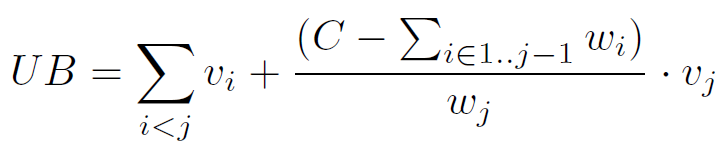
\includegraphics[width=0.5\linewidth]{KnapsackBBLinearRelaxationUB.png}
    \label{fig:Knapsack_example}
\end{figure}
\FloatBarrier

The search space is thus reduced as such :

\begin{figure}[!ht]
    \centering
    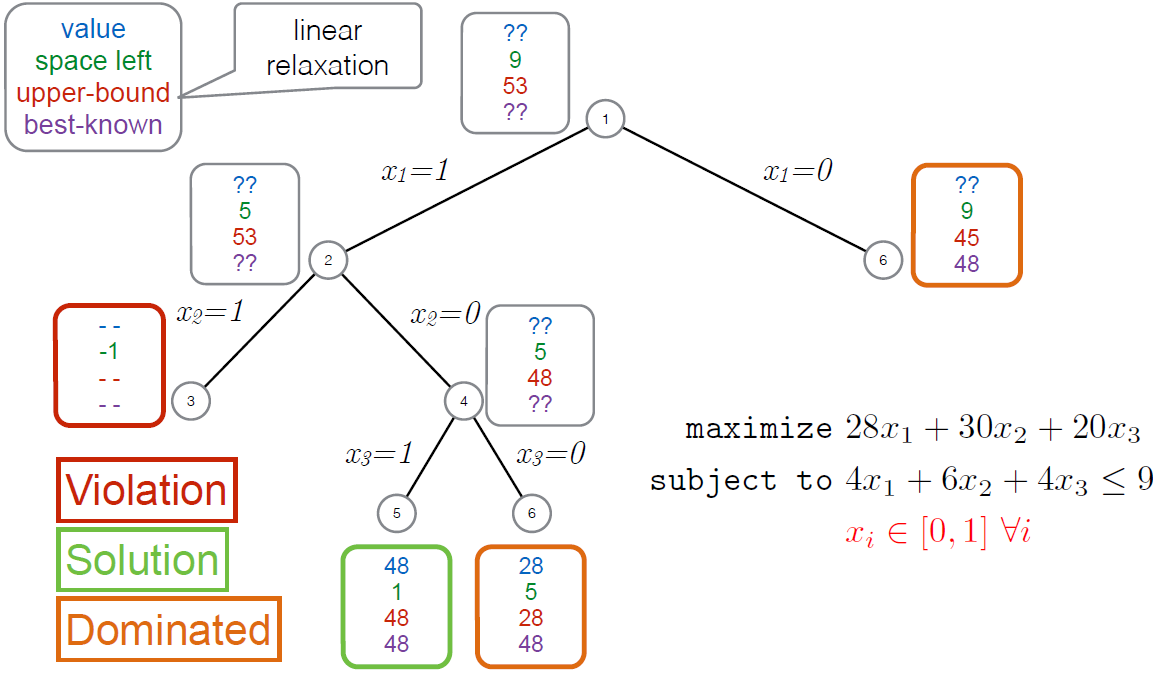
\includegraphics[width=\linewidth]{KnapsackBBLinearRelaxation.png}
    \label{fig:Knapsack_example}
\end{figure}
\FloatBarrier

As you can see, improving the precision of the upper-bound yields far better result. Take care however not to over/under estimate it (depending if you are on a maximisation or minimisation process) as it might prevent you to find the optimal solution.


